\newpage
\usecasebase{Visualizzazione dati utente}
\label{usecase:Visualizzazione dati utente}

\begin{figure}[h]
	\centering
	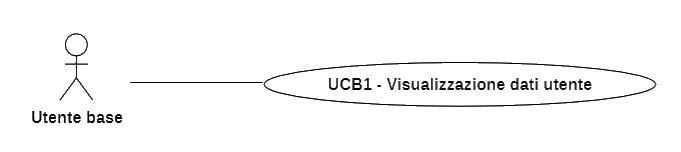
\includegraphics[width=0.8\textwidth]{./uml/UCB1.png} 
	\caption{Visualizzazione dati utente}
	\label{fig:UCB1}
  \end{figure}


\begin{itemize}
	\item \textbf{Attore principale:} Utente base.

	\item \textbf{Precondizioni:}
	      \begin{itemize}
		      \item L'Utente ha eseguito correttamente l'accesso al Sistema come
		            Utente base (vedi \autoref{usecase:Effettua accesso}).
		      \item L'Utente base si trova nella propria Area personale$^G$.
	      \end{itemize}

	\item \textbf{Postcondizione:} L'Utente base visualizza i propri dati utente.

	\item \textbf{Scenario principale:}
	      \begin{enumerate}
		      \item L'Utente base accede alla sezione Area personale e sceglie di visualizzare i suoi dati personali;
		      \item Il Sistema presenta all'Utente base le seguenti informazioni:
		            \begin{itemize}
			            \item Nome.
			            \item Cognome.
			            \item \textit{E-mail}.
			            \item \textit{Password}.
			            \item Dettagli sulle allergie e intolleranze.
		            \end{itemize}
	      \end{enumerate}
\end{itemize}
